\section{Introduction}
\label{sec:intro}



Graphs are an essential abstraction for a wide range of problems.  There are 
many ways to represent algorithms over graphs.  One class of methods defines
graphs in terms of matrices.  For example, we can define a graph in terms of an 
adjacency matrix where the rows and columns are labeled by the vertices and the
non-zero elements of the matrix are the edges between vertices.  

Expressing graph algorithms in the ``language of linear
algebra''~\cite{kepner2011graph} is a mature subject.  Multiple 
high performance graph libraries based on sparse 
linear algebra~\cite{combblas,
gadepally2015graphulo, gpi2016, sundaram2015graphmat,che2016programming}
have been developed.   With this ``Graphs as Linear Algebra'' approach established, 
a community of researchers came together to define common building
blocks for graphs expressed in the language of linear algebra.  They launched
this effort with a position paper~\cite{hpec13} in 2013 and formed the GraphBLAS
Forum~\cite{graphblas_web}.  After almost three years of steady work,
the GraphBLAS forum completed the
mathematical formalizations of the GraphBLAS~\cite{mathgraphblas16}. With another 
one and a half years of work, the group completed the C
language binding to the GraphBLAS~\cite{cspec}.

Currently there are multiple implementations of the GraphBLAS C specification.  
We have learned a great deal about how to define the operations within the GraphBLAS 
and how to implement them efficiently.  We are now ready to launch the next phase of the project:
to produce a library of high level graph algorithms implemented on top of the GraphBLAS.
We call this library of algorithms \emph{LAGraph}.
Just as we launched the GraphBLAS project with a position paper, we are launching 
this next phase of the project with a position paper.  

The goals of the LAGraph effort include, first and foremost, to bring together the full 
range of known graph algorithms that can be constructed with the GraphBLAS.
From this collection we will be able to systematically asses the coverage of 
graph algorithms based on linear algebra. This will also serve
as raw material in ongoing studies of the fundamental design patterns exploited 
by linear algebra-based graph algorithms. 

The basic outline of the LAGraph project  is summarized in 
Figure~\ref{fig:overview}. The library of algorithms is the single box towards
the middle of the figure.  These algorithms use the GraphBLAS C API
which exists as a separate implementation for a wide range of hardware
targets at the bottom of the figure.  To motivate our work and stay aligned 
with the way data scientists work with graph algorithms, we need to appreciate that
people will use a wide range of languages to access the graph algorithms.  A good library
must be able to work whether called directly from C or indirectly through a wrapper in Python.
Furthermore, the developers of the graph algorithm libraries will need a test harness to
validate the algorithms, I/O utilities, and a build system.  All of these components must
be addressed as part of the LAGraph project. 

Initially, LAGraph is not intended to be a production-worthy library of 
high level graph algorithms.  We expect over time, however, that from the LAGraph 
effort, we will produce such a library.  Anticipating that goal, we are constructing
the library ``as if'' it was to be used by data analytics end-users. That is, by people
who need the results from graph algorithms with little concern for how they are
implemented.  This requirement of building a library for \emph{end-users} as opposed to 
a library for \emph{graph algorithm researchers} has far reaching implications for the 
design of this software.

\begin{figure}[t]
	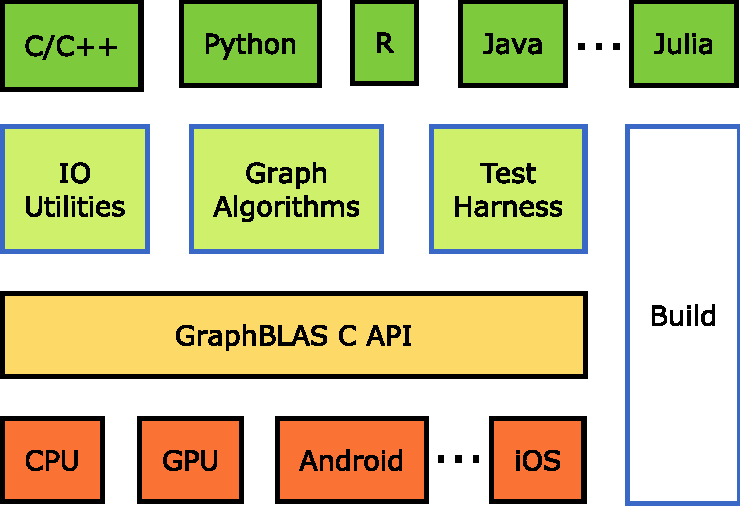
\includegraphics[width=\linewidth]{fig/lagraph}
	\caption{\textbf{LAGraph Project Overview.} The project consists of a library of 
	graph algorithms, assorted components to support algorithm development and validation
	(a test harness and I/O utilities) and it must interface to a wide range of languages.
	underneath these components is a build system, implementations of the GraphBLAS, 
	and a variety of hardware targets. \label{fig:overview}}
\end{figure}

We start the paper with a brief summary of the objects and operations defined in
the C specification of the GraphBLAS.  We then  summarize some of the 
early libraries that implement the GraphBLAS C specification.  Next, we describe
the repository where we will build LAGraph.  This is important since the
purpose of a position paper is to attract a community of researchers to join the effort
which means we want people to understand how to work with and perhaps contribute 
algorithms to the repository.  We then discuss the challenges we faced in writing the 
early version LAGraph and what it suggests about future developments needed in the
GraphBLAS themselves. We close with concluding remarks.














